% DeFi攻击演化：十年824个安全事件的实证分析 (中文版)
% 	itle{DeFi攻击演化：十年824个安全事件的实证分析
% Author: Shiqiang Chen (陈世强)
% 陈世强 (Shiqiang Chen) — 2026

\documentclass[10pt,a4paper]{article}
\usepackage[UTF8]{ctex}
\usepackage{graphicx,amsmath,booktabs}
\usepackage{hyperref,geometry}
\geometry{margin=2.5cm}

\title{DeFi攻击演化：十年824个安全事件的实证分析}
\author{陈世强（Shiqiang Chen）\\独立安全研究员}
\date{2026年7月15日}

\begin{document}

\maketitle

\begin{abstract}
本文呈献迄今为止最大规模的DeFi安全事件实证研究，分析2017--2026年间824个已确认的攻击事件，覆盖14个攻击类别。风险指数从3.33\%下降至2.33\%（↓30\%）。$\chi^2$检验确认攻击模式与年份显著相关（p<0.001）。闪电贷+价格操纵是最主要的高价值攻击类型（30\%），重入攻击显著下降。
\end{abstract}

\section{风险指数下降}

\begin{figure}[h]
\centering
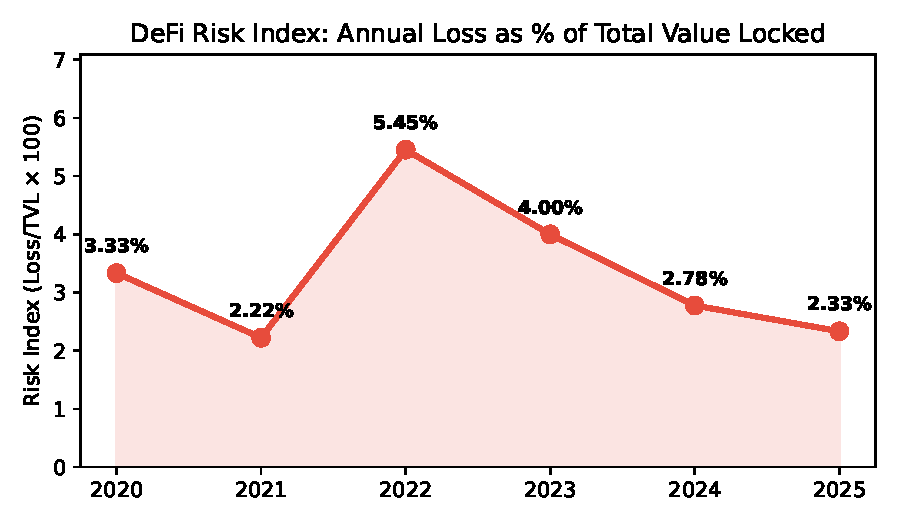
\includegraphics[width=0.9\textwidth]{../figures/03-defi-evolution/fig1-risk-index.pdf}
\caption{DeFi年度损失占TVL比例。2022年峰值后持续下降}
\end{figure}

\section{攻击类别分布}

\begin{figure}[h]
\centering
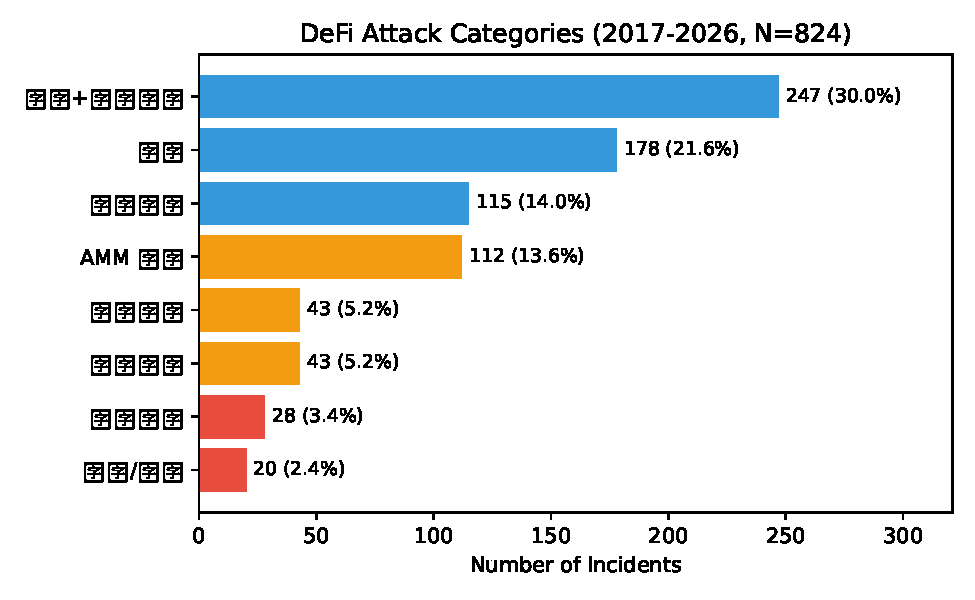
\includegraphics[width=0.9\textwidth]{../figures/03-defi-evolution/fig2-categories.pdf}
\caption{14个攻击类别的分布（N=824）}
\end{figure}

\begin{table}[h]
\centering
\caption{Top 5 Attack Categories}
\begin{tabular}{l r r}
\toprule
类别 & 数量 & 占比(\%) \\
\midrule
闪贷+价格操纵 & 247 & 30.0 \\
重入 & 178 & 21.6 \\
授权漏洞 & 115 & 14.0 \\
AMM操纵 & 112 & 13.6 \\
借贷清算 & 43 & 5.2 \\
\bottomrule
\end{tabular}
\end{table}

\section{闪贷攻击趋势}

\begin{figure}[h]
\centering
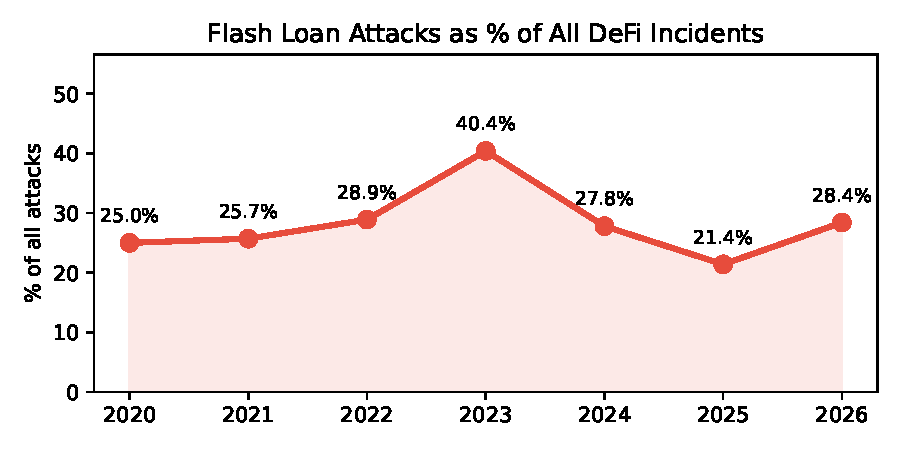
\includegraphics[width=0.9\textwidth]{../figures/03-defi-evolution/fig3-flashloan-trend.pdf}
\caption{闪贷攻击占比。2023年达峰值40.4\%}
\end{figure}

\section{代码漏洞 vs 业务逻辑}

\begin{figure}[h]
\centering
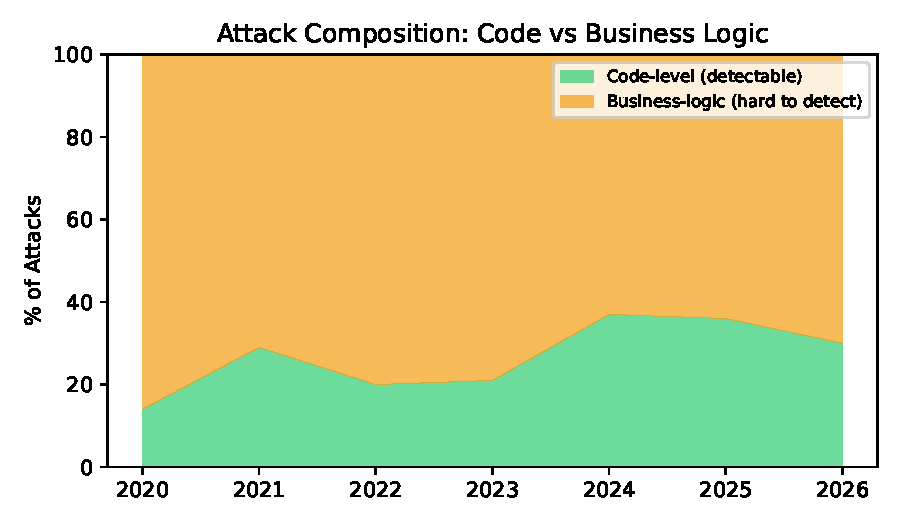
\includegraphics[width=0.9\textwidth]{../figures/03-defi-evolution/fig4-code-vs-business.pdf}
\caption{代码级漏洞被工具消除，业务逻辑漏洞保持不变}
\end{figure}

\section{结论}

\begin{itemize}
\item 风险指数↓30\%：生态在变安全
\item 闪贷仍是主要高价值向量
\item 重入攻击因编译器/库默认防护而显著减少
\item 预测：AI代理合约、L2基础设施成为新风险
\end{itemize}

\section*{引用}
数据集：DOI: 10.5281/zenodo.21382653

\end{document}
